\documentclass[aspectratio=169,10pt]{beamer}

\usetheme{default}
\usecolortheme{default}
\usefonttheme{professionalfonts}

\usepackage[utf8]{inputenc}
\usepackage[T1]{fontenc}
\usepackage[spanish]{babel}
\usepackage{graphicx}
\usepackage{booktabs}
\usepackage{tabularx}
\usepackage{adjustbox}
\usepackage{tikz}
\usepackage[table]{xcolor}
\usepackage{array}
\usepackage{ragged2e}

\graphicspath{{artifacts/figures/generated/}}

\definecolor{Navy}{HTML}{12355B}
\definecolor{Blue}{HTML}{1D74F5}
\definecolor{Teal}{HTML}{18A999}
\definecolor{Mint}{HTML}{E7F8F4}
\definecolor{Sky}{HTML}{EAF2FF}
\definecolor{Ink}{HTML}{14213D}
\definecolor{Muted}{HTML}{6B7280}
\definecolor{Paper}{HTML}{F8FAFC}
\definecolor{Warn}{HTML}{F59E0B}
\definecolor{Good}{HTML}{10B981}
\definecolor{Bad}{HTML}{EF4444}

\setbeamertemplate{navigation symbols}{}
\setbeamertemplate{itemize item}{\color{Blue}\small$\blacktriangleright$}
\setbeamercolor{normal text}{fg=Ink,bg=white}
\setbeamercolor{frametitle}{fg=Navy,bg=white}
\setbeamerfont{frametitle}{series=\bfseries,size=\Large}
\setbeamertemplate{frametitle}{
  \vspace{0.22cm}
  \begin{beamercolorbox}[wd=\paperwidth,leftskip=0.55cm,rightskip=0.55cm]{frametitle}
    \insertframetitle
  \end{beamercolorbox}
  \vspace{-0.18cm}
}

\setbeamertemplate{footline}{
  \begin{tikzpicture}[remember picture,overlay]
    \fill[Paper] (current page.south west) rectangle ([yshift=0.27cm]current page.south east);
    \fill[Blue] (current page.south west) rectangle ([xshift=\paperwidth,yshift=0.04cm]current page.south west);
    \node[anchor=south east, font=\scriptsize, text=Muted] at ([xshift=-0.35cm,yshift=0.07cm]current page.south east) {\insertframenumber};
  \end{tikzpicture}
}

\newcommand{\slidemeta}[2]{
  \vfill
  {\scriptsize\color{Muted}\textbf{Tiempo} #1 \hfill \textbf{Mensaje clave} #2}
}

\newcommand{\pill}[2]{
  \tikz[baseline=(x.base)] \node[rounded corners=6pt, fill=#1, text=white, inner xsep=6pt, inner ysep=3pt] (x) {\scriptsize\bfseries #2};
}

\title{Sistema de apoyo al analisis inicial de casos ante el TEDH}
\subtitle{Clasificacion multietiqueta, retrieval de precedentes y auditoria}
\author{Mauro Valls Vidal}
\institute{Grado en Ingenieria en Inteligencia Artificial\\Aprendizaje Avanzado\\Universidad de Alicante}
\date{}

\begin{document}

% -------------------------------------------------------------------
\begin{frame}[plain]
  \begin{tikzpicture}[remember picture,overlay]
    \fill[Sky] (current page.south west) rectangle (current page.north east);
    \fill[Navy] (current page.south west) rectangle ([xshift=0.45\paperwidth]current page.north west);
    \node[anchor=west, text=white, align=left, text width=0.38\paperwidth] at ([xshift=0.65cm]current page.west) {
      {\LARGE\bfseries Sistema de apoyo al analisis inicial de casos ante el TEDH}\\[0.25cm]
      {\normalsize Clasificacion multietiqueta, precedentes y auditoria}\\[0.35cm]
      \pill{Teal}{Clasificar} \quad \pill{Blue}{Recuperar} \quad \pill{Warn}{Auditar}\\[0.45cm]
      {\small Mauro Valls Vidal}\\
      {\scriptsize Aprendizaje Avanzado · Universidad de Alicante}
    };
    \node[anchor=center] at ([xshift=0.24\paperwidth]current page.center) {
      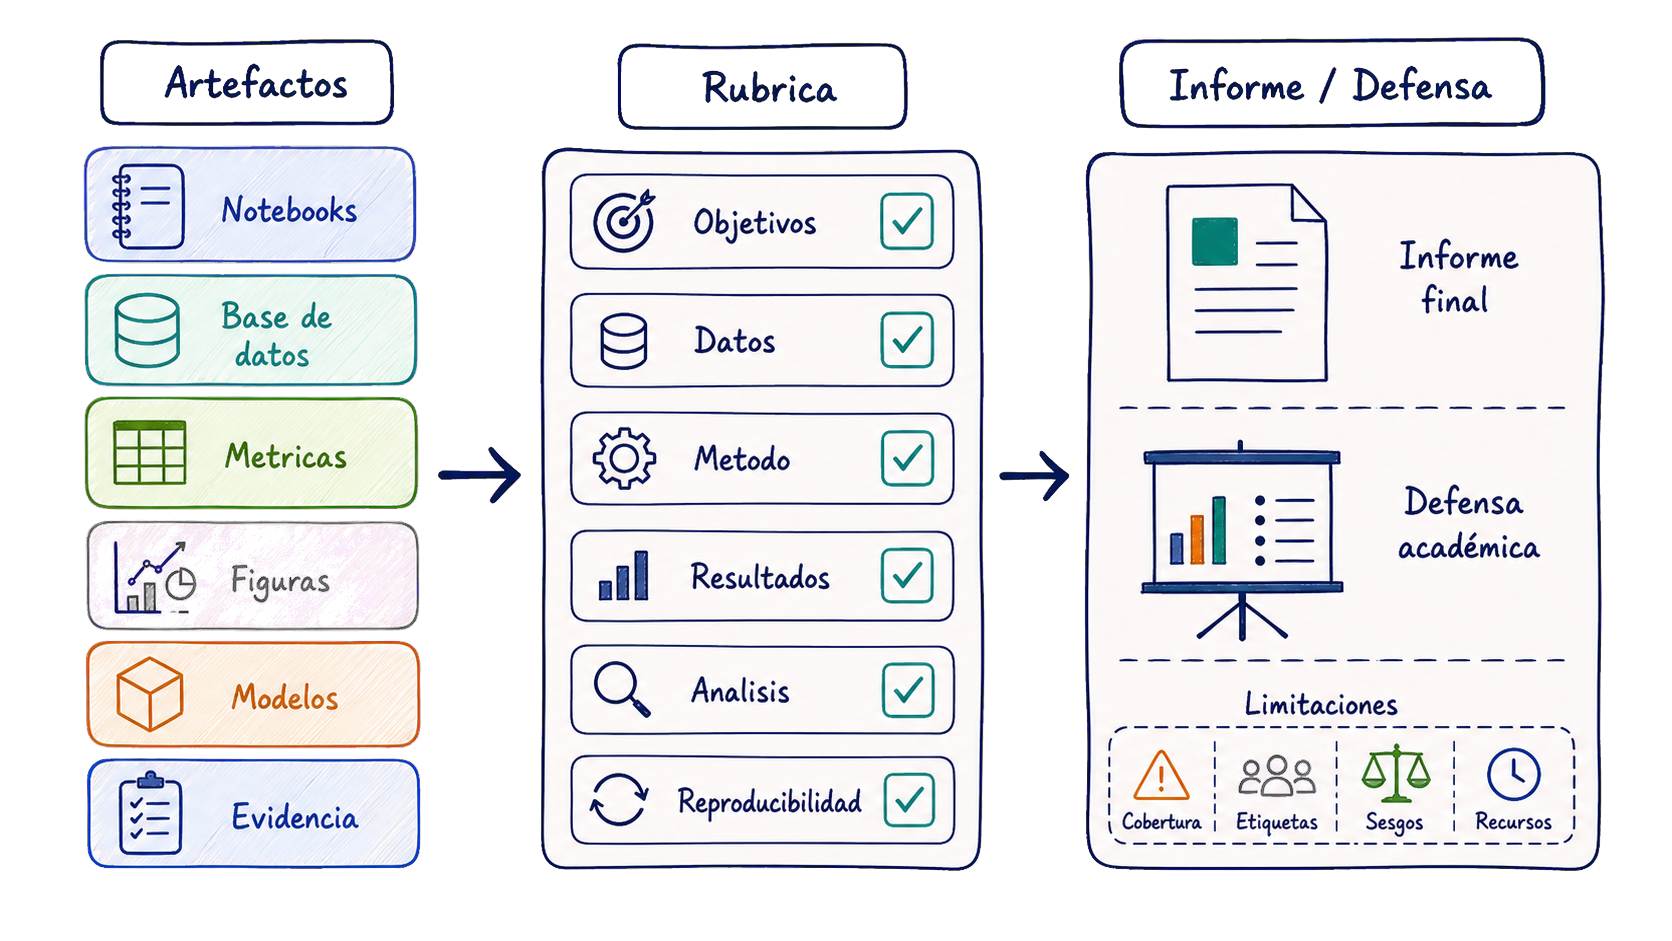
\includegraphics[width=0.49\paperwidth,height=0.70\paperheight,keepaspectratio]{notebook_05_evidence_v2.png}
    };
  \end{tikzpicture}
  % IMAGEN GENERADA RECOMENDADA PARA PORTADA
  % Prompt. Modern professional presentation cover for a European Court of Human Rights case analysis assistant, courthouse silhouette, legal documents, clean data flow lines, human decision support, blue and teal palette, elegant university defense style, no text.
  % NOTAS DEL PRESENTADOR
  % Tiempo recomendado 40 segundos.
  % Abrir con la idea principal. Este proyecto no automatiza decisiones juridicas. Construye un sistema reproducible que ayuda a priorizar articulos, precedentes y auditoria.
\end{frame}

% -------------------------------------------------------------------
\begin{frame}{Problema real}
  \begin{columns}[T,onlytextwidth]
    \column{0.58\textwidth}
    \textbf{Analizar un caso TEDH es costoso}
    \begin{itemize}
      \item Hay que detectar articulos posibles.
      \item Hay que revisar precedentes y evitar omisiones.
      \item Textos largos y juridicamente densos.
      \item Varios articulos pueden aparecer juntos.
      \item Un falso negativo puede ocultar una linea de revision.
    \end{itemize}
    \column{0.38\textwidth}
    \begin{block}{Idea clave}
      El sistema sugiere.\\
      \textbf{La persona decide.}
    \end{block}
    \vspace{0.15cm}
    \begin{tabular}{lr}
      \toprule
      Casos & 11000\\
      Articulos & 10\\
      Pares positivos & 15991\\
      \bottomrule
    \end{tabular}
  \end{columns}
  \slidemeta{1 min}{El sistema es apoyo, no sustitucion}
  % IMAGEN GENERADA RECOMENDADA PARA HUMANO EN EL BUCLE
  % Prompt. A legal analyst reviewing suggested legal articles on a clean dashboard, human in the loop, responsible AI support, legal documents, modern Google Slides style, blue teal palette, no text.
  % NOTAS DEL PRESENTADOR
  % Explicar el contexto. En una revision inicial de un caso TEDH, el analista debe leer hechos largos, detectar articulos posibles y buscar precedentes.
  % La herramienta no decide. Ordena informacion y reduce carga de lectura.
  % La frase clave es "el sistema sugiere, la persona decide".
\end{frame}

% -------------------------------------------------------------------
\begin{frame}{Objetivo del sistema}
  \begin{enumerate}
    \item \textbf{Sugerir articulos candidatos} para apoyar el analisis inicial.
    \item \textbf{Recuperar precedentes similares} dentro del conjunto de entrenamiento.
    \item \textbf{Auditar resultados y errores} mediante metricas, explicabilidad y revision de fallos.
  \end{enumerate}
  \vspace{0.35cm}
  \begin{block}{Criterio del proyecto}
    El objetivo no es ganar una metrica aislada. El objetivo es construir un flujo util, reproducible y revisable.
  \end{block}
  \slidemeta{45 s}{Tres salidas forman un sistema completo}
  % NOTAS DEL PRESENTADOR
  % Presentar la defensa como una historia. Primero clasificamos articulos, luego buscamos precedentes y finalmente auditamos comportamiento.
  % Estas tres piezas justifican que el proyecto sea mas que un clasificador.
\end{frame}

% -------------------------------------------------------------------
\begin{frame}{Ejemplo real de uso auditado}
  \small
  \begin{tabularx}{\linewidth}{>{\bfseries}p{0.23\linewidth}X}
    \toprule
    Entrada & Caso test real \texttt{ecthr\_task\_b\_test\_000000}. Texto de hechos con 4774 tokens.\\
    Prediccion auditada & Articulo 10. Score LogReg 0.9605.\\
    Explicacion local & Terminos LIME relevantes: \texttt{journalist}, \texttt{broadcasting}, \texttt{journalists}, \texttt{press}.\\
    Uso humano & Revisar, confirmar o descartar las sugerencias.\\
    \bottomrule
  \end{tabularx}
  \vspace{0.28cm}
  \begin{block}{Advertencia}
    La salida es una sugerencia revisable, no una conclusion juridica.
  \end{block}
  {\scriptsize\color{Muted}Ejemplo extraido de \texttt{04\_xai\_drift\_y\_errores.ipynb}.}
  \slidemeta{1 min}{El ejemplo muestra trazabilidad, no razonamiento juridico}
  % NOTAS DEL PRESENTADOR
  % Este ejemplo sale de los notebooks revisados. En 02_modelado_multilabel aparece el caso ecthr_task_b_test_000000 con articulo 10 positivo y 4774 tokens.
  % En 04_xai_drift_y_errores aparece una explicacion LIME para el articulo 10 con score 0.960473 y terminos como journalist, broadcasting, journalists y press.
  % Los notebooks de retrieval revisados muestran metricas agregadas, pero no un identificador concreto de precedente recuperado para este caso. Por eso no se inventa ningun precedente especifico.
  % Este caso no se presenta como prueba juridica. Se usa para mostrar trazabilidad: entrada, prediccion y explicacion local.
  % La decision final siempre queda en manos de una persona experta.
\end{frame}

% -------------------------------------------------------------------
\begin{frame}{Dataset}
  \begin{columns}[T,onlytextwidth]
    \column{0.45\textwidth}
    \begin{adjustbox}{width=\linewidth}
    \begin{tabular}{lr}
      \toprule
      \textbf{Elemento} & \textbf{Valor}\\
      \midrule
      Train & 9000\\
      Validation & 1000\\
      Test & 1000\\
      Total & 11000\\
      Articulos & 10\\
      Pares positivos & 15991\\
      Parrafos & 262580\\
      \bottomrule
    \end{tabular}
    \end{adjustbox}
    \column{0.50\textwidth}
    \begin{itemize}
      \item \textbf{Entrada:} texto de hechos de casos del TEDH.
      \item \textbf{Salida:} vector de 10 articulos posibles.
      \item Un mismo caso puede activar varios articulos.
      \item Train selecciona hiperparametros con CV.
      \item Test se reserva para la evaluacion final.
    \end{itemize}
  \end{columns}
  \slidemeta{1 min}{El dataset encaja con una tarea multietiqueta}
  % NOTAS DEL PRESENTADOR
  % Decir que LexGLUE ECtHR Task B ya trae particiones oficiales. No mezclamos los splits.
  % Train se usa para GridSearchCV con 5 folds. Test se guarda para medir rendimiento final.
  % Lo importante es que la salida no es una clase unica. Es un vector con 10 decisiones binarias.
\end{frame}

% -------------------------------------------------------------------
\begin{frame}{Protocolo de evaluacion}
  \begin{columns}[T,onlytextwidth]
    \column{0.50\textwidth}
    \begin{block}{Seleccion}
      \begin{itemize}
        \item \texttt{GridSearchCV}
        \item Validacion cruzada de 5 folds
        \item Solo con \texttt{train}
        \item Macro-F1 como metrica principal
      \end{itemize}
    \end{block}
    \column{0.46\textwidth}
    \begin{block}{Evaluacion final}
      \begin{itemize}
        \item TF-IDF dentro de \texttt{Pipeline}
        \item SVD y scaler dentro del \texttt{Pipeline}
        \item Refit con todo \texttt{train}
        \item \texttt{test} solo al final
      \end{itemize}
    \end{block}
  \end{columns}
  \vspace{0.25cm}
  \begin{block}{Regla clave}
    Test no ajusta hiperparametros, umbrales, arquitectura ni seleccion de modelo.
  \end{block}
  \slidemeta{1.25 min}{El test queda reservado para la comparativa final}
  % NOTAS DEL PRESENTADOR
  % Esta diapositiva responde directamente al criterio nuevo del profesor.
  % GridSearchCV se ejecuta sobre train con 5 folds. El vectorizador TF-IDF forma parte del Pipeline, por lo que se ajusta dentro de cada fold sin ver los datos de validacion interna.
  % Tras elegir hiperparametros, refit=True reentrena el mejor estimador con todo train.
  % Test solo se usa para la evaluacion final y la comparativa de modelos.
\end{frame}

% -------------------------------------------------------------------
\begin{frame}{EDA y dificultad}
  \begin{columns}[T,onlytextwidth]
    \column{0.58\textwidth}
    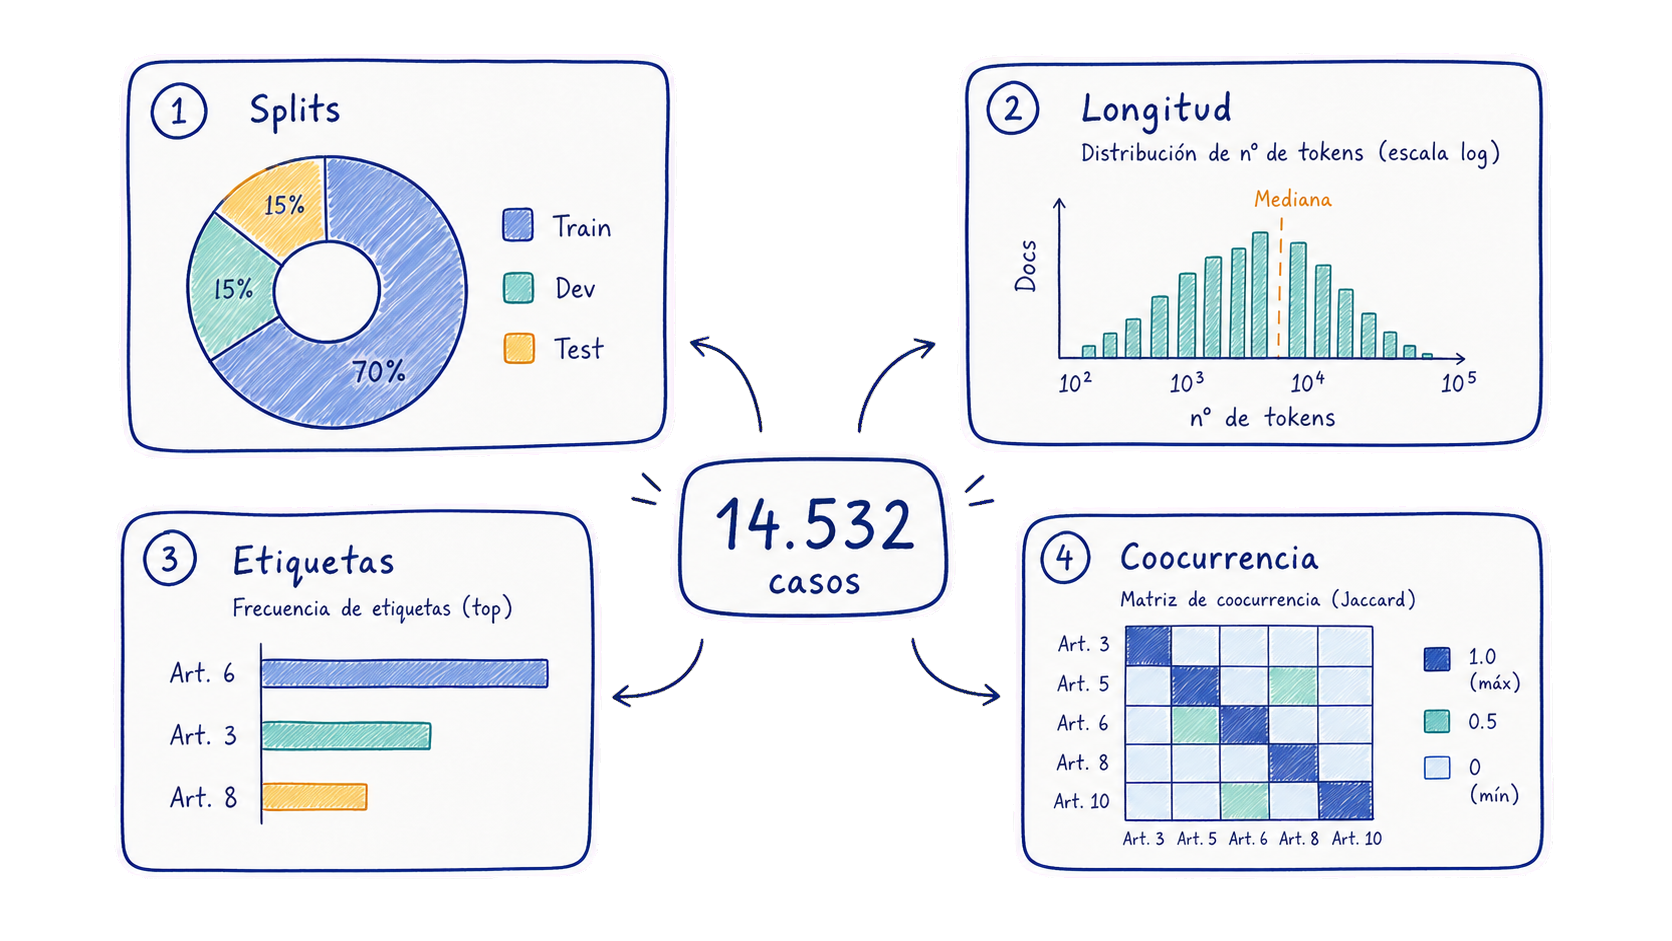
\includegraphics[width=\linewidth,height=0.70\paperheight,keepaspectratio]{notebook_01_eda_v2.png}
    \column{0.38\textwidth}
    \begin{itemize}
      \item Articulo 6 domina con 6225 casos.
      \item Articulo 9 solo tiene 101 casos.
      \item Hay documentos de hasta 35780 tokens.
      \item Hay coocurrencias entre articulos.
    \end{itemize}
    \vspace{0.18cm}
    \begin{block}{Lectura}
      El reto combina longitud, desbalanceo y varios articulos por caso.
    \end{block}
  \end{columns}
  \slidemeta{1 min}{La dificultad viene de longitud, desbalanceo y coocurrencias}
  % NOTAS DEL PRESENTADOR
  % La imagen resume el EDA. La lectura oral debe conectar tres problemas.
  % Primero, los documentos son largos. Segundo, el articulo 6 domina y puede sesgar el aprendizaje. Tercero, varios articulos coocurren.
  % El reto no es solo clasificar textos, sino hacerlo con documentos largos, etiquetas desbalanceadas y multiples articulos por caso.
  % Por eso accuracy no seria una metrica suficiente y usamos macro-F1, micro-F1 y Hamming loss.
\end{frame}

% -------------------------------------------------------------------
\begin{frame}{Matrices X e Y}
  \begin{columns}[T,onlytextwidth]
    \column{0.57\textwidth}
    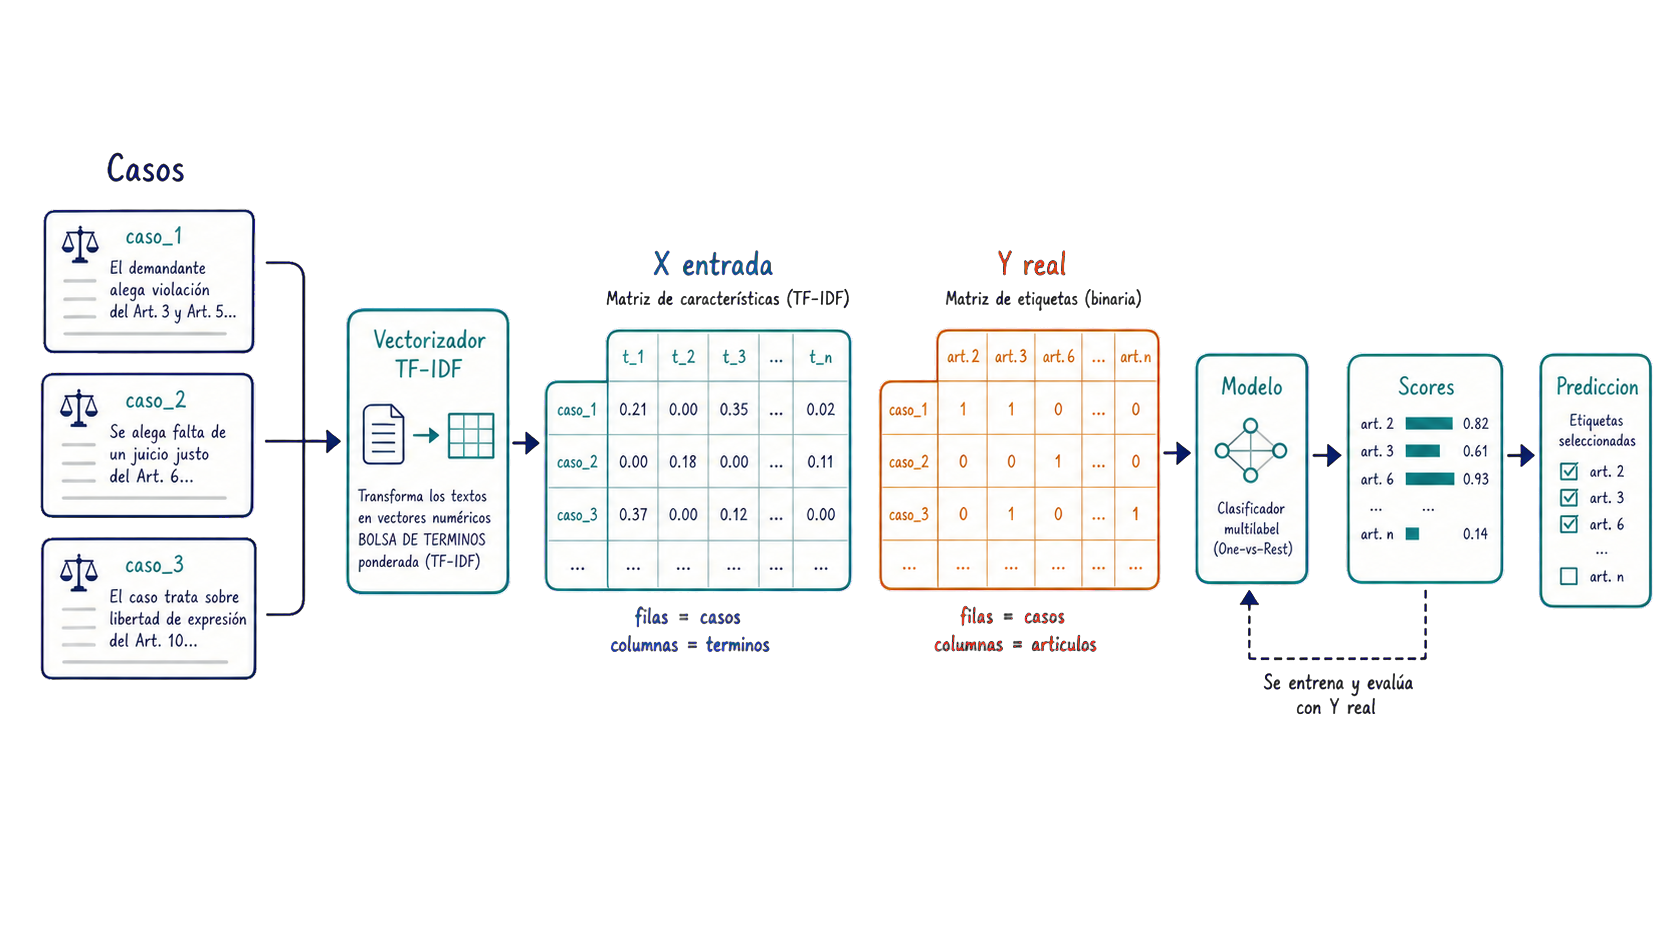
\includegraphics[width=\linewidth,height=0.70\paperheight,keepaspectratio]{notebook_02_xy_matrix_flow_v2.png}
    \column{0.39\textwidth}
    \begin{itemize}
      \item \textbf{X:} texto convertido en pesos TF-IDF.
      \item \textbf{Y:} matriz binaria de 10 articulos.
      \item \textbf{One-vs-Rest:} 10 clasificadores binarios, uno por articulo.
      \item Esta formulacion permite varias etiquetas por caso.
    \end{itemize}
  \end{columns}
  \slidemeta{1 min}{Un caso puede activar varios articulos}
  % NOTAS DEL PRESENTADOR
  % X es la matriz de entrada. Cada fila es un caso y cada columna representa un termino o bigrama ponderado.
  % Y es la matriz de salida. Cada fila tiene 10 posiciones. Puede haber mas de un 1.
  % One-vs-Rest encaja porque no obligamos al modelo a elegir un unico articulo. Entrenamos una decision binaria por articulo.
\end{frame}

% -------------------------------------------------------------------
\begin{frame}{Ingesta y SQLite}
  \begin{columns}[T,onlytextwidth]
    \column{0.60\textwidth}
    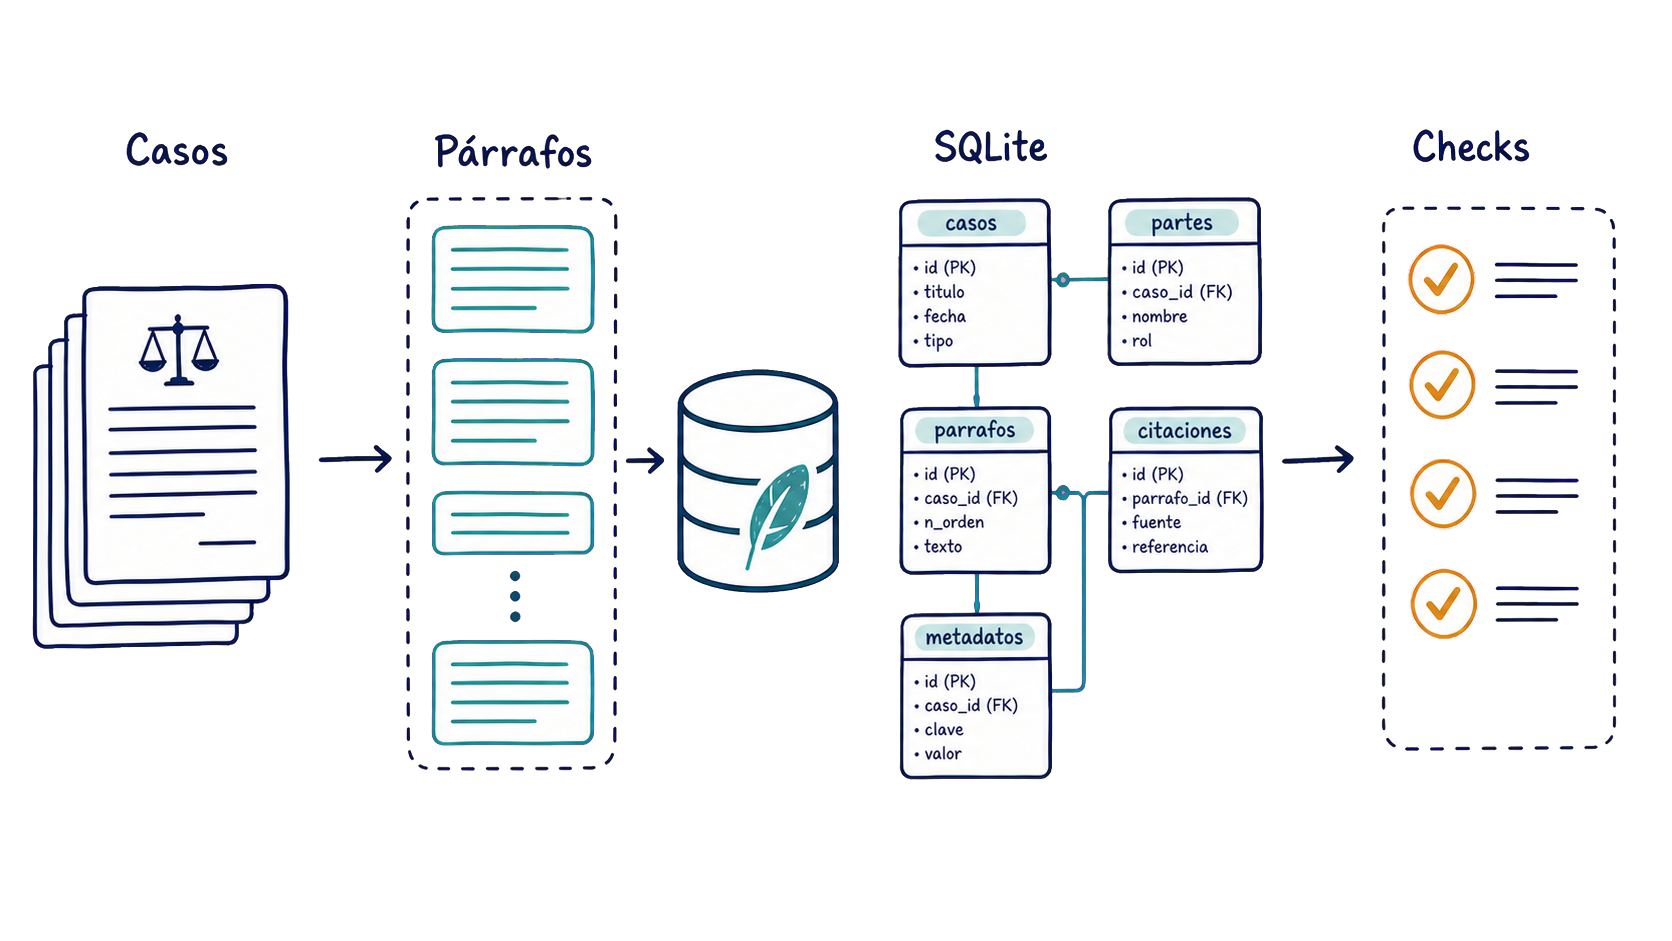
\includegraphics[width=\linewidth,height=0.70\paperheight,keepaspectratio]{notebook_00_ingestion_schema_v2.png}
    \column{0.36\textwidth}
    \begin{itemize}
      \item Casos, parrafos y etiquetas quedan separados.
      \item La trazabilidad se conserva por \texttt{case\_id}.
      \item Predicciones y explicaciones se pueden guardar.
      \item El pipeline se puede regenerar.
    \end{itemize}
  \end{columns}
  \slidemeta{1 min}{SQLite da orden y reproducibilidad}
  % NOTAS DEL PRESENTADOR
  % Explicar que la base SQLite no es un detalle tecnico menor. Es lo que permite ordenar casos, parrafos, articulos, etiquetas y predicciones.
  % Esto facilita reproducibilidad y evita trabajar con ficheros sueltos.
\end{frame}

% -------------------------------------------------------------------
\begin{frame}{Pipeline completo}
  \begin{center}
    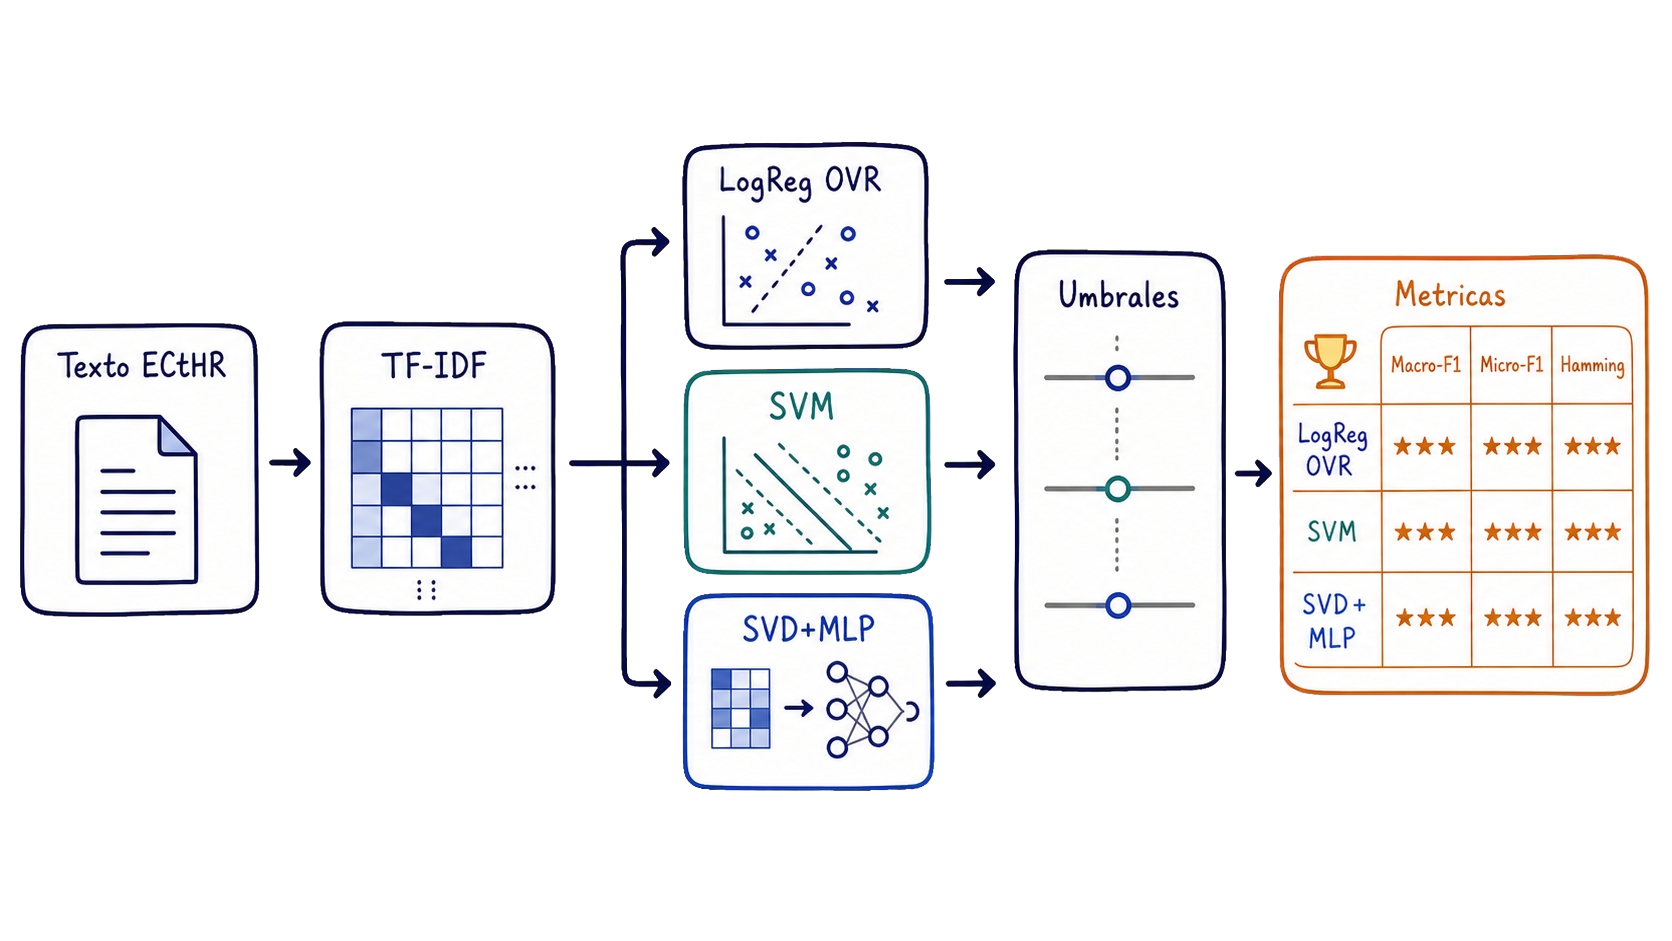
\includegraphics[width=0.82\linewidth,height=0.52\paperheight,keepaspectratio]{notebook_02_modeling_v2.png}
  \end{center}
  \vspace{-0.05cm}
  \small
  \begin{itemize}
    \item \textbf{TF-IDF:} pesa terminos frecuentes en un caso y no comunes en todo el corpus.
    \item \textbf{One-vs-Rest:} diez decisiones binarias, una por articulo.
      \item \textbf{GridSearchCV:} selecciona hiperparametros con 5 folds sobre train.
  \end{itemize}
  \slidemeta{1.25 min}{El Pipeline evita leakage durante la validacion cruzada}
  % NOTAS DEL PRESENTADOR
  % TF-IDF transforma cada caso en un vector de pesos de terminos. Da mas importancia a palabras frecuentes en un documento pero no frecuentes en todo el corpus.
  % En dominio juridico esto ayuda porque palabras como detention, hearing o property pueden estar asociadas a articulos concretos.
  % One-vs-Rest entrena 10 clasificadores binarios. Esto encaja con el problema porque un caso puede tener varios articulos.
  % La parte importante del protocolo nuevo es que TF-IDF esta dentro del Pipeline. En cada fold se ajusta solo con la parte de entrenamiento del fold.
\end{frame}

% -------------------------------------------------------------------
\begin{frame}{Modelos evaluados}
  \begin{tabularx}{\linewidth}{>{\bfseries}p{0.27\linewidth}X}
    \toprule
    Baseline & Predice siempre la etiqueta mas frecuente. Sirve como punto de partida.\\
    LogReg OVR & Modelo auditado con coeficientes interpretables.\\
    SVM lineal OVR & Mejor rendimiento final en test.\\
    SVD + MLP & Comparacion secundaria con reduccion de dimensionalidad y rejilla pequena.\\
    \bottomrule
  \end{tabularx}
  \vspace{0.25cm}
  \begin{block}{Decision metodologica}
    Se prioriza una solucion clasica por reproducibilidad, bajo coste computacional y auditoria directa.
  \end{block}
  \slidemeta{45 s}{Se compara rendimiento y capacidad de auditoria}
  % NOTAS DEL PRESENTADOR
  % Esta diapositiva prepara la comparacion. El baseline marca un suelo. LogReg es interpretable. SVM es fuerte para texto disperso. MLP aparece como comparacion, no como nucleo.
  % TF-IDF y modelos lineales pueden ser menos potentes que modelos profundos, pero son mas transparentes y faciles de reproducir.
  % En este proyecto la interpretabilidad y la trazabilidad forman parte del objetivo, no son un complemento.
  % Los modelos juridicos largos o LLMs quedan como trabajo futuro o comparacion posterior.
\end{frame}

% -------------------------------------------------------------------
\begin{frame}{Como leer las metricas}
  \small
  \begin{tabularx}{\linewidth}{>{\bfseries}p{0.22\linewidth}X}
    \toprule
    Macro-F1 & Rendimiento medio por etiqueta. Es importante porque hay articulos minoritarios.\\
    Micro-F1 & Rendimiento global agregando todos los aciertos y errores.\\
    Hamming loss & Proporcion de decisiones caso-articulo incorrectas. Mas bajo es mejor.\\
    Recall@10 & Indica si aparece al menos un precedente relevante entre los 10 primeros.\\
    nDCG@10 & Mide si los precedentes relevantes aparecen bien posicionados en el ranking.\\
    \bottomrule
  \end{tabularx}
  \vspace{0.25cm}
  \begin{block}{Lectura rapida}
    Para clasificacion miramos especialmente Macro-F1 y Hamming loss. Para retrieval miramos Recall@10.
  \end{block}
  \slidemeta{1 min}{Las metricas responden preguntas distintas}
  % NOTAS DEL PRESENTADOR
  % Esta diapositiva evita que las tablas parezcan numeros sueltos.
  % Macro-F1 mira cada etiqueta por separado y despues promedia. Es clave por el desbalanceo.
  % Micro-F1 resume rendimiento global. Hamming loss mide errores por cada decision caso-articulo.
  % En retrieval, Recall@10 responde si el top 10 contiene algun caso relevante. nDCG@10 mira si los relevantes aparecen arriba.
\end{frame}

% -------------------------------------------------------------------
\begin{frame}{LogReg frente a SVM}
  \begin{adjustbox}{width=\linewidth}
    \begin{tabular}{lrrrrl}
      \toprule
      \textbf{Modelo} & \textbf{Split} & \textbf{Macro-F1} & \textbf{Micro-F1} & \textbf{Hamming} & \textbf{Lectura}\\
      \midrule
      LogReg OVR & CV train & 0.726 & -- & -- & Modelo auditable\\
      SVM lineal & CV train & 0.733 & -- & -- & Mejor CV\\
      LogReg OVR & test & 0.736 & 0.760 & 0.069 & Modelo auditado\\
      \rowcolor{Mint}
      SVM lineal & test & 0.749 & 0.777 & 0.061 & Mejor rendimiento\\
      \bottomrule
    \end{tabular}
  \end{adjustbox}
  \vspace{0.25cm}
  \begin{block}{Lectura}
    SVM obtiene el mejor rendimiento final. LogReg se mantiene para auditoria porque sus coeficientes se interpretan mejor.
  \end{block}
  \slidemeta{1.5 min}{SVM gana en test, LogReg gana en auditoria}
  % NOTAS DEL PRESENTADOR
  % No ocultar que SVM es el mejor modelo por rendimiento final. En test mejora macro-F1 y Hamming frente a LogReg.
  % La razon para mantener LogReg como modelo auditado no es que rinda mas en test. Es que permite revisar coeficientes y explicaciones locales con mas facilidad.
  % Respuesta preparada: SVM es el mejor modelo en rendimiento final de test. Por eso lo reportamos claramente. LogReg queda como modelo auditado porque sus coeficientes son mas interpretables.
  % Esta distincion es central. Rendimiento final y trazabilidad explicable son criterios distintos.
\end{frame}

% -------------------------------------------------------------------
\begin{frame}{Resultados de clasificacion}
  \begin{columns}[T,onlytextwidth]
    \column{0.52\textwidth}
    \begin{adjustbox}{width=\linewidth}
      \begin{tabular}{lrrr}
        \toprule
        \textbf{Modelo en test} & \textbf{Macro-F1} & \textbf{Micro-F1} & \textbf{Hamming}\\
        \midrule
        LogReg OVR & 0.736 & 0.760 & 0.069\\
        \rowcolor{Mint}
        SVM lineal & 0.749 & 0.777 & 0.061\\
        SVD + MLP & 0.690 & 0.767 & 0.062\\
        Baseline & 0.057 & 0.324 & 0.165\\
        \bottomrule
      \end{tabular}
    \end{adjustbox}
    \column{0.44\textwidth}
    \begin{block}{Mejor modelo en test}
      \begin{itemize}
        \item Macro-F1: \textbf{0.749}
        \item Micro-F1: \textbf{0.777}
        \item Hamming loss: \textbf{0.061}
      \end{itemize}
    \end{block}
    \small SVM mejora la macro-F1 y Hamming frente a LogReg. MLP no supera a los modelos lineales.
  \end{columns}
  \slidemeta{1.25 min}{La SVM lineal obtiene el mejor rendimiento en test}
  % NOTAS DEL PRESENTADOR
  % Que muestra la tabla. Compara los modelos en test, que es la evaluacion final.
  % La conclusion principal es que SVM lineal es el mejor modelo por rendimiento.
  % Macro-F1 es la metrica mas importante aqui porque hay etiquetas minoritarias.
  % La limitacion es que el buen rendimiento no permite automatizar decisiones juridicas. Es una herramienta de apoyo.
  % La tabla completa con train, validation y test queda en backup.
\end{frame}

% -------------------------------------------------------------------
\begin{frame}{Retrieval de precedentes}
  \begin{columns}[T,onlytextwidth]
    \column{0.46\textwidth}
    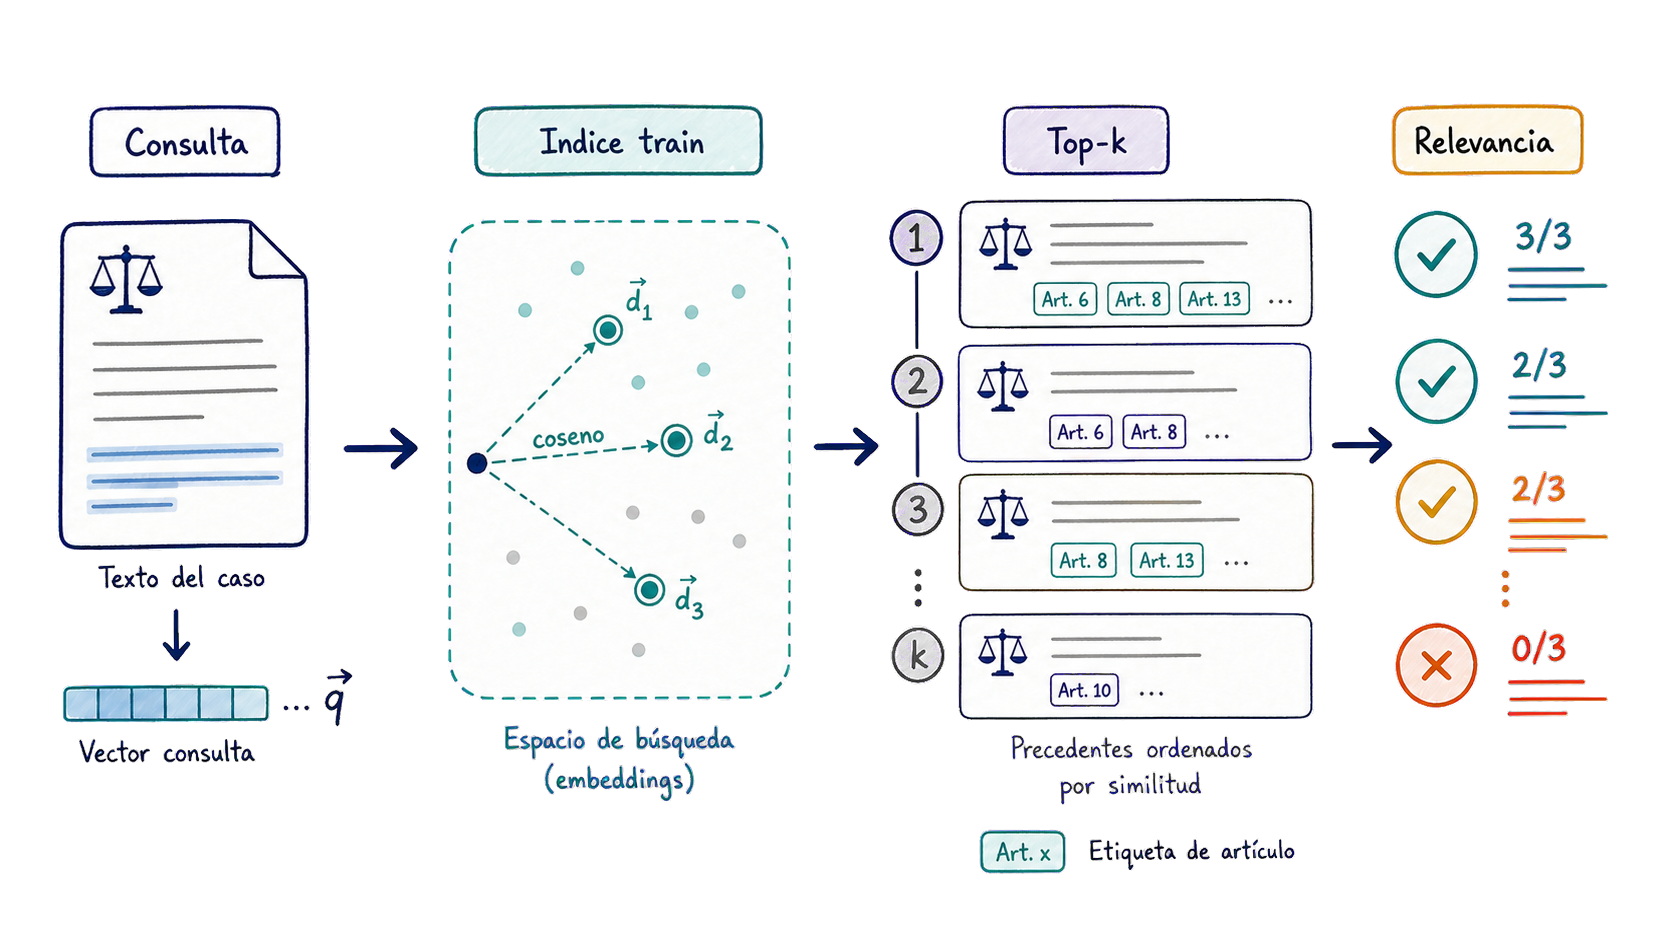
\includegraphics[width=\linewidth,height=0.66\paperheight,keepaspectratio]{notebook_03_retrieval_v2.png}
    \column{0.50\textwidth}
    \begin{adjustbox}{width=\linewidth}
      \begin{tabular}{llrrr}
        \toprule
        \textbf{Metodo} & \textbf{Split} & \textbf{R@5} & \textbf{R@10} & \textbf{nDCG}\\
        \midrule
        TF-IDF & validation & 0.952 & 0.964 & 0.882\\
        \rowcolor{Mint}
        TF-IDF & test & 0.944 & 0.972 & 0.867\\
        SVD & validation & 0.960 & 0.964 & 0.898\\
        SVD & test & 0.940 & 0.956 & 0.876\\
        \bottomrule
      \end{tabular}
    \end{adjustbox}
    \vspace{0.20cm}
    \small Un caso recuperado se considera relevante si comparte al menos un articulo real con la consulta.
  \end{columns}
  \slidemeta{1.25 min}{El top 10 suele contener precedentes con articulos compartidos}
  % NOTAS DEL PRESENTADOR
  % Una consulta es el caso que queremos analizar. El indice de train es el conjunto de casos candidatos ya conocidos.
  % La similitud coseno compara la orientacion de los vectores TF-IDF. Si dos casos usan vocabulario parecido, quedan cerca.
  % Top-k significa mirar los k primeros resultados del ranking.
  % La metrica principal es Recall@10. En test, TF-IDF coseno alcanza 0.972.
  % Limitacion importante. Compartir articulos es una aproximacion reproducible, pero no demuestra que el precedente sea doctrinalmente equivalente.
\end{frame}

% -------------------------------------------------------------------
\begin{frame}{Explicabilidad}
  \begin{columns}[T,onlytextwidth]
    \column{0.55\textwidth}
    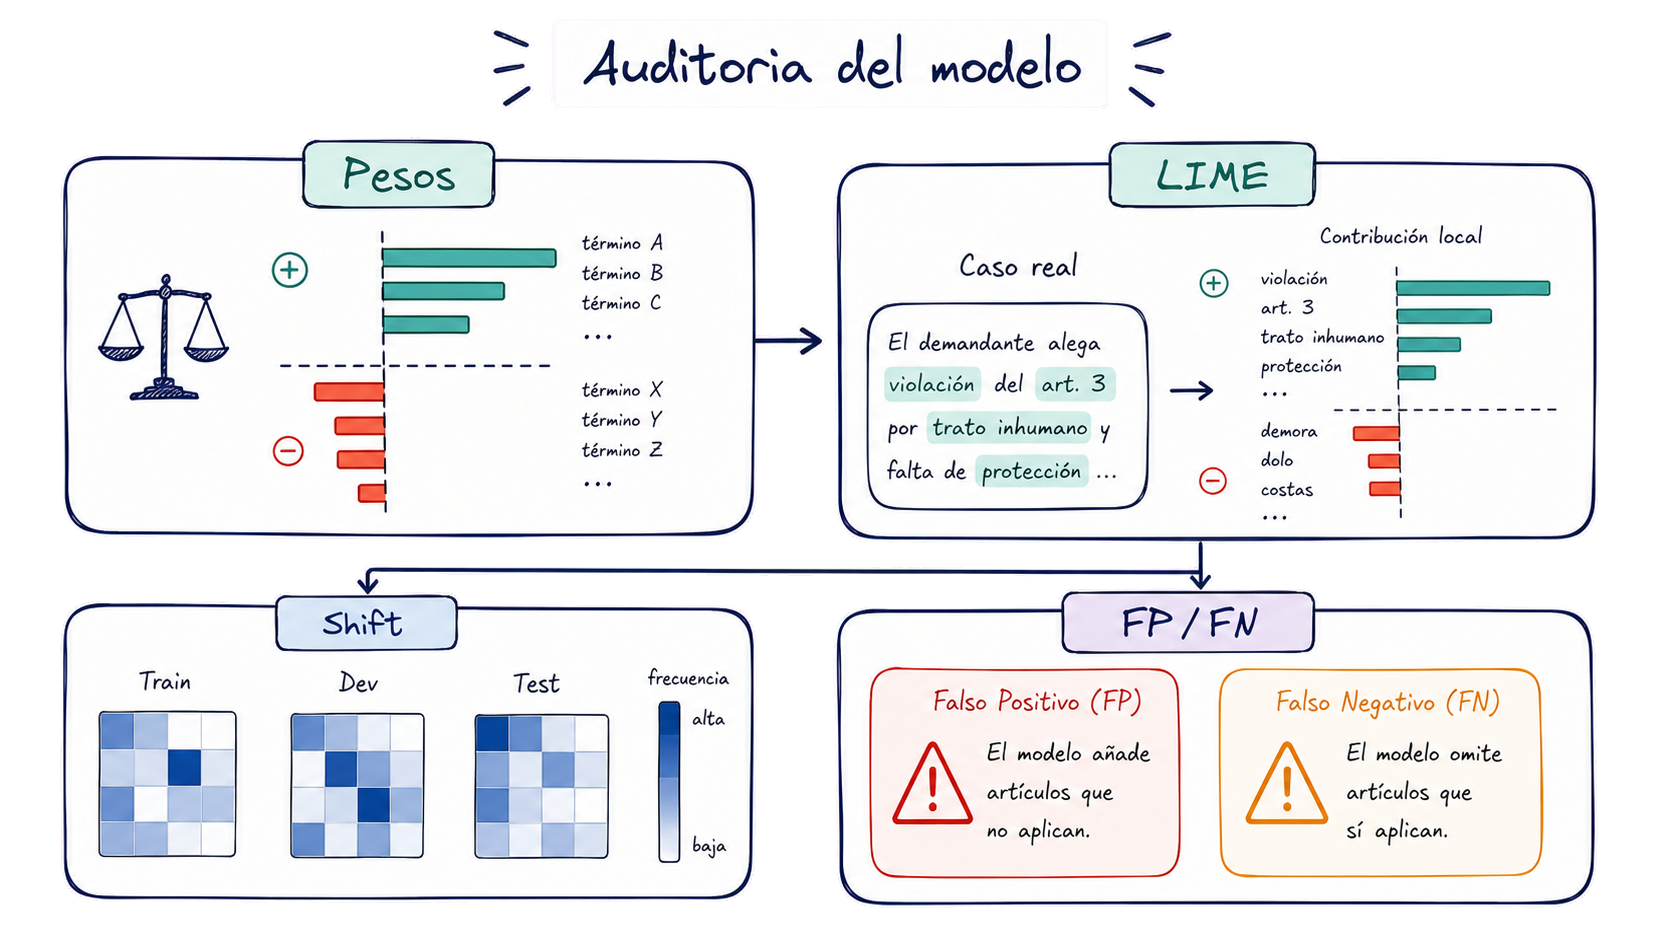
\includegraphics[width=\linewidth,height=0.68\paperheight,keepaspectratio]{notebook_04_audit_v2.png}
    \column{0.41\textwidth}
    \begin{itemize}
      \item \textbf{Global:} coeficientes por articulo.
      \item \textbf{Local:} LIME para revisar un caso concreto.
      \item \textbf{Auditoria:} shift, falsos positivos y falsos negativos.
      \item Las explicaciones no son pruebas juridicas.
    \end{itemize}
  \end{columns}
  \slidemeta{1 min}{Explicar el modelo no equivale a justificar juridicamente}
  % NOTAS DEL PRESENTADOR
  % La explicabilidad global usa coeficientes. Ayuda a ver que terminos pesan mas para cada articulo.
  % LIME es local. Permite revisar un caso concreto y ver que palabras influyen en esa prediccion.
  % Ejemplo real revisado. Para ecthr_task_b_test_000000 y articulo 10, LIME destaca terminos como journalist, press y broadcasting.
  % En la prueba de fidelidad, retirar journalist baja el score de 0.960473 a 0.944687. Esto sugiere influencia local, no una prueba juridica.
  % Como ejemplo conceptual, si terminos relacionados con detencion pesaran mucho para el articulo 5, eso permitiria revisar si el modelo se apoya en senales razonables.
  % Ninguno de los dos demuestra causalidad juridica. Son herramientas para auditar comportamiento estadistico del modelo.
\end{frame}

% -------------------------------------------------------------------
\begin{frame}{Shift entre particiones}
  \begin{adjustbox}{width=0.88\linewidth}
    \begin{tabular}{lrrrrrr}
      \toprule
      \textbf{Split} & \textbf{JS} & \textbf{L1} & \textbf{Coseno} & \(\Delta\)\textbf{Macro} & \(\Delta\)\textbf{Micro} & \(\Delta\)\textbf{Hamming}\\
      \midrule
      validation & 0.017 & 0.278 & 0.959 & 0.000 & 0.000 & 0.000\\
      test & 0.026 & 0.320 & 0.951 & 0.006 & -0.015 & 0.005\\
      \bottomrule
    \end{tabular}
  \end{adjustbox}
  \vspace{0.22cm}
  \small
  \begin{itemize}
    \item JS y L1 miden diferencias entre distribuciones de etiquetas.
    \item Coseno mide similitud de direccion entre distribuciones.
    \item Los deltas muestran cuanto cambia el rendimiento frente a validation.
  \end{itemize}
  \slidemeta{1 min}{Se mide shift entre particiones, no deriva temporal estricta}
  % NOTAS DEL PRESENTADOR
  % Jensen-Shannon mide diferencia entre distribuciones de etiquetas.
  % L1 mide distancia absoluta entre frecuencias. Coseno mide si las distribuciones apuntan en una direccion parecida.
  % Los deltas de F1 y Hamming muestran como cambia el rendimiento respecto a validation.
  % No afirmamos drift temporal estricto porque la version usada del dataset no expone ano oficial de sentencia.
\end{frame}

% -------------------------------------------------------------------
\begin{frame}{Errores FP y FN}
  \begin{columns}[T,onlytextwidth]
    \column{0.52\textwidth}
    \begin{adjustbox}{width=\linewidth}
      \begin{tabular}{rrrl}
        \toprule
        \textbf{FP} & \textbf{FN} & \textbf{Casos} & \textbf{Lectura}\\
        \midrule
        0 & 0 & 491 & Prediccion exacta\\
        1 & 0 & 189 & Carga extra\\
        0 & 1 & 170 & Articulo omitido\\
        1 & 1 & 65 & Mixto\\
        0 & 2 & 36 & Omision doble\\
        2 & 0 & 25 & Revision extra\\
        \bottomrule
      \end{tabular}
    \end{adjustbox}
    \column{0.42\textwidth}
    \begin{itemize}
      \item \textbf{FP:} sugiere un articulo que no aparece en la etiqueta real.
      \item Aumenta carga de revision.
      \item \textbf{FN:} no sugiere un articulo real.
      \item Puede ocultar una linea relevante.
    \end{itemize}
  \end{columns}
  \slidemeta{1 min}{En apoyo juridico, los FN son especialmente delicados}
  % NOTAS DEL PRESENTADOR
  % FP significa falso positivo. El sistema propone un articulo que no esta en la etiqueta real. Esto aumenta carga de revision.
  % FN significa falso negativo. El sistema no propone un articulo que si era real. Esto puede ocultar una linea juridica.
  % Por eso en una herramienta real podria estudiarse un ajuste de umbrales segun el coste de cada error. Ese ajuste no debe hacerse con test.
\end{frame}

% -------------------------------------------------------------------
\begin{frame}{Reproducibilidad}
  \begin{columns}[T,onlytextwidth]
    \column{0.58\textwidth}
    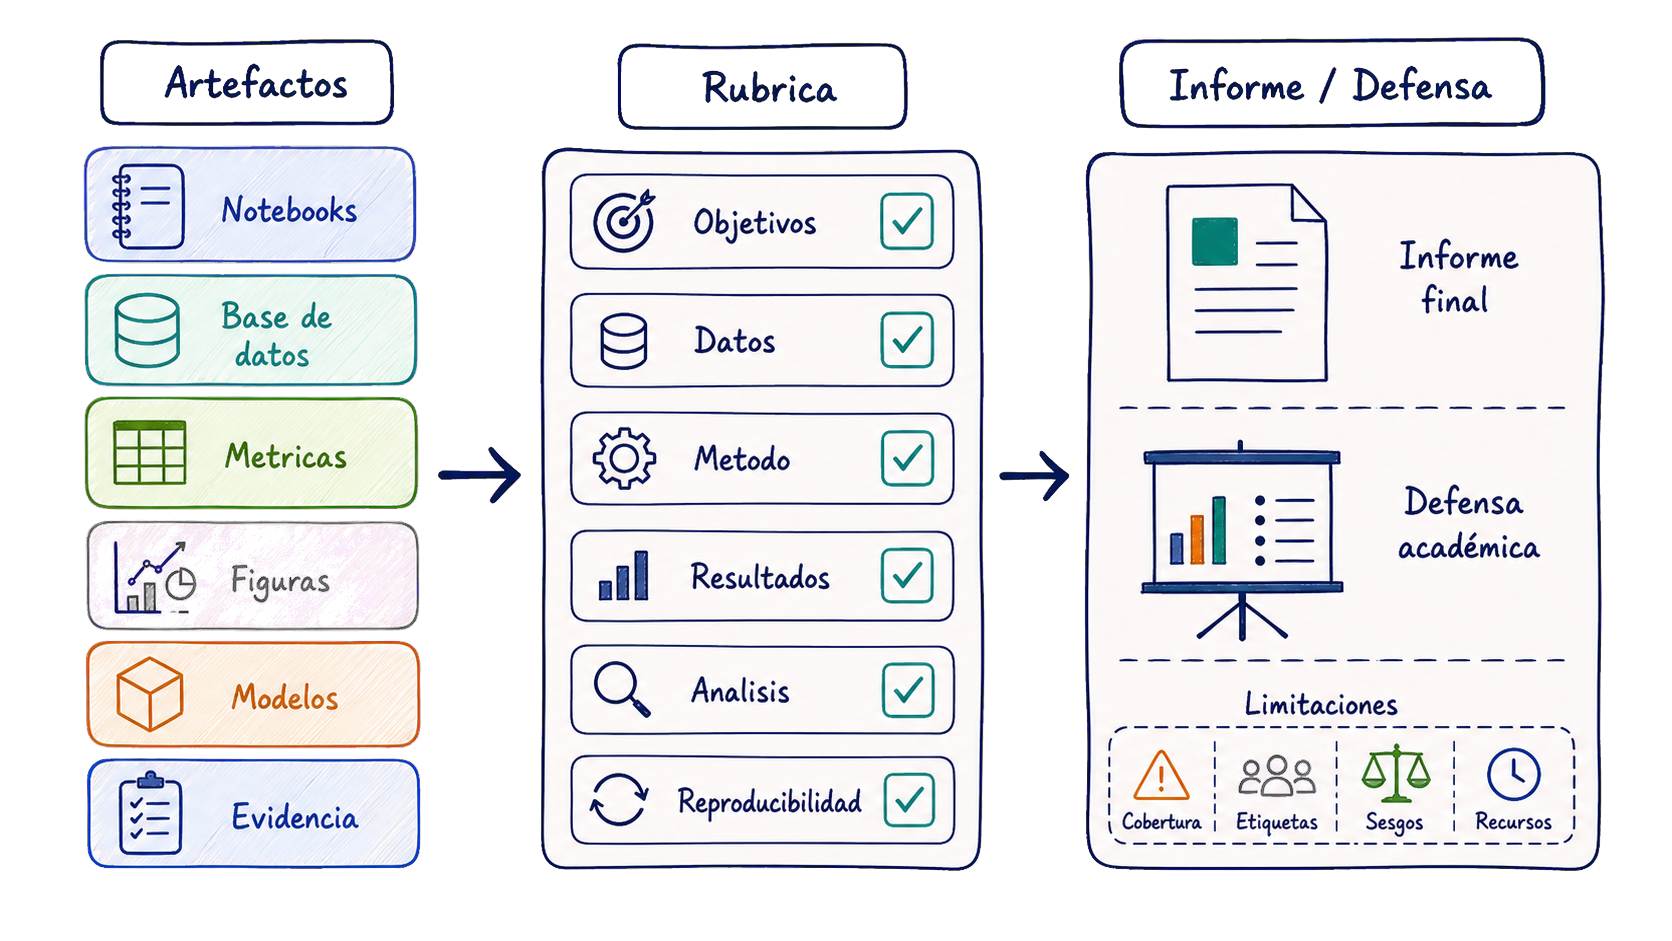
\includegraphics[width=\linewidth,height=0.70\paperheight,keepaspectratio]{notebook_05_evidence_v2.png}
    \column{0.38\textwidth}
    \begin{itemize}
      \item Notebooks numerados de 00 a 05.
      \item SQLite como base central.
      \item Semilla fija.
      \item Artefactos regenerables.
      \item Test reservado para evaluacion final.
    \end{itemize}
  \end{columns}
  \slidemeta{45 s}{La entrega se puede reconstruir paso a paso}
  % NOTAS DEL PRESENTADOR
  % Recalcar que no es solo una tabla de resultados. Hay una cadena completa desde ingesta hasta informe.
  % Tambien explicar data leakage. TF-IDF esta dentro de Pipeline y se ajusta dentro de cada fold. Test se reserva para la evaluacion final.
\end{frame}

% -------------------------------------------------------------------
\begin{frame}{Limitaciones}
  \begin{itemize}
    \item TF-IDF no capta toda la semantica juridica.
    \item Retrieval usa articulos compartidos como aproximacion de relevancia.
    \item Las explicaciones no son pruebas juridicas.
    \item No hay validacion cualitativa por juristas de los precedentes recuperados.
  \end{itemize}
  \vspace{0.25cm}
  \begin{block}{Uso responsable}
    El sistema requiere supervision humana. Su salida es una ayuda de priorizacion, no una decision automatica.
  \end{block}
  \slidemeta{1 min}{Reconocer limites hace mas responsable el sistema}
  % NOTAS DEL PRESENTADOR
  % Explicar las limitaciones sin debilitar el trabajo.
  % El modelo aprende patrones textuales del benchmark. No interpreta normas como un jurista.
  % Retrieval usa una definicion operativa de relevancia. LIME y coeficientes ayudan a auditar, pero no prueban causalidad.
  % Tambien falta validacion cualitativa por juristas de los precedentes recuperados. Por eso una mejora natural es evaluar esos precedentes con expertos juridicos.
  % Esto refuerza el encuadre responsable del proyecto.
\end{frame}

% -------------------------------------------------------------------
\begin{frame}{Trabajo futuro}
  \begin{columns}[T,onlytextwidth]
    \column{0.48\textwidth}
    \begin{itemize}
      \item Evaluacion cualitativa de precedentes con juristas.
      \item Calibracion de probabilidades.
      \item Umbrales segun coste de error.
    \end{itemize}
    \column{0.48\textwidth}
    \begin{itemize}
      \item Comparacion controlada con modelos juridicos largos.
      \item Monitorizacion de shift y degradacion.
      \item Protocolo de privacidad para datos sensibles.
    \end{itemize}
  \end{columns}
  \slidemeta{45 s}{La mejora principal esta en validacion humana y control de riesgo}
  % NOTAS DEL PRESENTADOR
  % Presentar estas mejoras como extension natural, no como carencias graves.
  % Lo mas importante seria validar precedentes con expertos y ajustar umbrales segun coste de error.
\end{frame}

% -------------------------------------------------------------------
\begin{frame}{Conclusion}
  \begin{itemize}
    \item Clasifica articulos candidatos en una tarea multietiqueta.
    \item Recupera precedentes similares con un criterio reproducible.
    \item Audita senales, shift y patrones de error.
  \end{itemize}
  \vspace{0.35cm}
  \begin{block}{Aportacion final}
    La aportacion no es automatizar el derecho, sino priorizar la revision juridica de forma reproducible y auditable.
  \end{block}
  \slidemeta{1 min}{Un sistema de apoyo, no una automatizacion juridica}
  % IMAGEN GENERADA RECOMENDADA PARA CIERRE
  % Prompt. Three connected actions classify retrieve audit, legal documents and data flow, human supervised legal AI assistant, modern professional presentation illustration, blue teal palette, no text.
  % NOTAS DEL PRESENTADOR
  % Cerrar con una frase clara. El proyecto convierte casos largos en tres ayudas revisables.
  % Clasificar no basta. Un sistema juridico util tambien debe recuperar evidencia, mostrar sus limites y permitir auditoria humana.
  % SVM aporta el mejor rendimiento. LogReg aporta auditoria. Retrieval y errores completan la vision responsable.
\end{frame}

% -------------------------------------------------------------------
\appendix
\begin{frame}{Backup. Tabla completa de clasificacion}
  \begin{adjustbox}{width=\linewidth}
    \begin{tabular}{llrrrr}
      \toprule
      \textbf{Modelo} & \textbf{Split} & \textbf{Casos} & \textbf{Macro-F1} & \textbf{Micro-F1} & \textbf{Hamming}\\
      \midrule
      LogReg OVR & train & 9000 & 0.908 & 0.923 & 0.023\\
      LogReg OVR & validation & 1000 & 0.730 & 0.775 & 0.064\\
      LogReg OVR & test & 1000 & 0.736 & 0.760 & 0.069\\
      SVM lineal & validation & 1000 & 0.732 & 0.791 & 0.057\\
      \rowcolor{Mint}
      SVM lineal & test & 1000 & 0.749 & 0.777 & 0.061\\
      SVD + MLP & validation & 1000 & 0.698 & 0.776 & 0.060\\
      SVD + MLP & test & 1000 & 0.690 & 0.767 & 0.062\\
      \bottomrule
    \end{tabular}
  \end{adjustbox}
  % NOTAS DEL PRESENTADOR
  % Backup por si preguntan por validation o MLP. No es necesario mostrarla en la exposicion principal si no hay tiempo.
\end{frame}

\begin{frame}{Backup. Preguntas de defensa I}
  \footnotesize
  \begin{tabularx}{\linewidth}{>{\bfseries}p{0.31\linewidth}X}
      \toprule
      Pregunta & Respuesta breve\\
      \midrule
      El sistema decide que articulos se han vulnerado & No. Sugiere articulos candidatos y precedentes para priorizar la revision. La decision juridica queda en manos de una persona experta.\\
      Por que GridSearchCV & Porque permite comparar configuraciones con el mismo protocolo y sin mirar test.\\
      Por que 5-fold CV & Porque reduce dependencia de una sola particion interna de train y es el criterio pedido por el profesor.\\
      Por que solo train para seleccionar & Porque test debe quedar limpio para estimar rendimiento final.\\
      Por que TF-IDF & Es reproducible, eficiente con textos largos y permite inspeccionar terminos.\\
      Por que no usar directamente un modelo profundo o LLM & Porque el objetivo no era solo maximizar rendimiento, sino construir un sistema reproducible, auditable y explicable. Los modelos profundos pueden compararse en trabajo futuro.\\
      Por que es multietiqueta & Un caso puede estar asociado a varios articulos a la vez.\\
      Que significa Macro-F1 & F1 medio por etiqueta. Es importante por las etiquetas minoritarias.\\
      Que significa Micro-F1 & F1 global agregando aciertos y errores.\\
      Por que SVM gana pero LogReg se audita & SVM rinde mejor en test. LogReg permite revisar coeficientes de forma directa.\\
      \bottomrule
  \end{tabularx}
  % NOTAS DEL PRESENTADOR
  % Usar esta diapositiva como apoyo si el profesor pregunta por metodologia, metricas o decision de modelo.
\end{frame}

\begin{frame}{Backup. Preguntas de defensa II}
  \footnotesize
  \begin{tabularx}{\linewidth}{>{\bfseries}p{0.31\linewidth}X}
      \toprule
      Pregunta & Respuesta breve\\
      \midrule
      Que limitacion tiene LIME & Explica localmente el modelo, pero no demuestra causalidad juridica.\\
      La explicacion LIME justifica legalmente la prediccion & No. LIME ayuda a inspeccionar que terminos influyen localmente en el modelo, pero no demuestra causalidad ni sustituye una argumentacion juridica.\\
      El caso mostrado demuestra que el modelo razona juridicamente & No. Demuestra trazabilidad y capacidad de auditoria. El modelo detecta patrones textuales asociados a etiquetas, pero no interpreta normas como un jurista.\\
      Que significa shift entre particiones & Cambio de distribucion entre train, validation y test, no deriva temporal estricta.\\
      Riesgo de falsos negativos & Pueden ocultar articulos relevantes y reducir la revision humana.\\
      Como se evita data leakage & TF-IDF esta dentro de Pipeline y se ajusta dentro de cada fold. Test se reserva para evaluar.\\
      Por que test no ajusta nada & Porque test debe medir rendimiento final sin influir en decisiones.\\
      Que haria antes de desplegarlo en un entorno real & Validacion por juristas, calibracion de probabilidades, ajuste de umbrales por coste de error, control de privacidad y monitorizacion de degradacion.\\
      Que mejoraria & Validacion experta, calibracion, umbrales por coste, privacidad y modelos juridicos largos.\\
      \bottomrule
  \end{tabularx}
  % NOTAS DEL PRESENTADOR
  % Usar esta diapositiva como apoyo si el profesor pregunta por XAI, riesgos, despliegue o trabajo futuro.
\end{frame}

\begin{frame}{Backup. Prompts visuales recomendados}
  \small
  \begin{itemize}
    \item Portada. ``Modern professional presentation cover for a European Court of Human Rights case analysis assistant, courthouse silhouette, legal documents, clean data flow lines, human decision support, blue and teal palette, elegant university defense style, no text.''
    \item Humano en el bucle. ``A legal analyst reviewing suggested legal articles on a clean dashboard, human in the loop, responsible AI support, legal documents, modern Google Slides style, blue teal palette, no text.''
    \item Falso negativo. ``Conceptual visualization of a relevant legal article hidden behind a stack of case documents, showing risk of missed issue, subtle amber warning accent, clean legal tech presentation style, no text.''
    \item Cierre. ``Three connected actions classify retrieve audit, legal documents and data flow, human supervised legal AI assistant, modern professional presentation illustration, blue teal palette, no text.''
  \end{itemize}
  % NOTAS DEL PRESENTADOR
  % Estos prompts son opcionales. No son necesarios para compilar.
\end{frame}

\end{document}